
    \begin{center}
        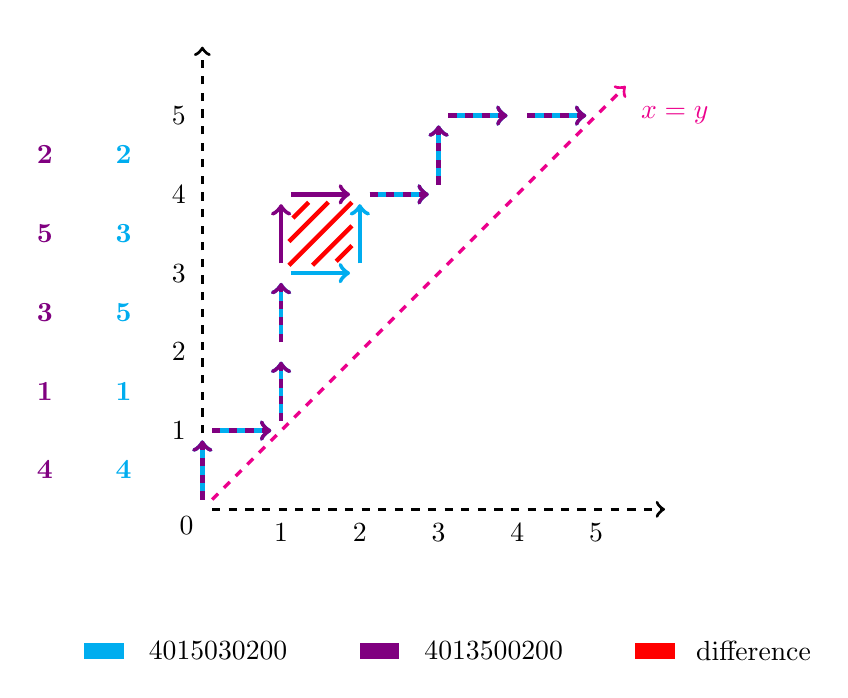
\begin{tikzpicture}[scale=1]
            \node (a) at (0, 0) {};
            \node (b) at (0, 6) {};
            \node (c) at (6, 0) {};
            \node (d) at (5.5, 5.5) {};
            \node (e) at (6, 5) [color = magenta]
                {$x = y$}; 
            \draw [dashed, very thick, ->] (a) to (b);
            \draw [dashed, very thick, ->] (a) to (c);
            \draw [dashed, very thick, ->]
                [color = magenta] (a) to (d);

            \node (1)  at (0,0)   {};
            \node (2)  at (0,1)   {};
            \node (3)  at (1,1)   {};
            \node (4)  at (1,2)   {};
            \node (5)  at (1,3)   {};
            \node (6)  at (2,3)   {};
            \node (6b) at (1,4)   {};
            \node (7)  at (2,4)   {};
            \node (8)  at (3,4)   {};
            \node (9)  at (3,5)   {};
            \node (10) at (4,5)   {};
            \node (11) at (5,5)   {};

            \draw [->, ultra thick, color = cyan]
                (1)  to (2);
            \draw [->, ultra thick, color = cyan] 
                (2)  to (3);
            \draw [->, ultra thick, color = cyan]
                (3)  to (4);
            \draw [->, ultra thick, color = cyan]
                (4)  to (5);
            \draw [->, ultra thick, color = cyan]
                (5)  to (6);
            \draw [->, ultra thick, color = cyan]
                (6)  to (7);
            \draw [->, ultra thick, color = cyan]
                (7)  to (8);
            \draw [->, ultra thick, color = cyan]
                (8)  to (9);
            \draw [->, ultra thick, color = cyan]
                (9)  to (10);
            \draw [->, ultra thick, color = cyan]
                (10) to (11);

            \draw [->, dashed, ultra thick, color = violet]
                (1)  to (2);
            \draw [->, dashed, ultra thick, color = violet] 
                (2)  to (3);
            \draw [->, dashed, ultra thick, color = violet]
                (3)  to (4);
            \draw [->, dashed, ultra thick, color = violet]
                (4)  to (5);
            \draw [->, ultra thick, color = violet]
                (5)  to (6b);
            \draw [->, ultra thick, color = violet]
                (6b)  to (7);
            \draw [->, dashed, ultra thick, color = violet]
                (7)  to (8);
            \draw [->, dashed, ultra thick, color = violet]
                (8)  to (9);
            \draw [->, dashed, ultra thick, color = violet]
                (9)  to (10);
            \draw [->, dashed, ultra thick, color = violet]
                (10) to (11);

            \node at (-0.2, -0.2) {$0$};
            \node at (-0.3, 1)    {$1$};
            \node at (1, -0.3)    {$1$};
            \node at (-0.3, 2)    {$2$};
            \node at (2, -0.3)    {$2$};
            \node at (-0.3, 3)    {$3$};
            \node at (3, -0.3)    {$3$};
            \node at (-0.3, 4)    {$4$};
            \node at (4, -0.3)    {$4$};
            \node at (-0.3, 5)    {$5$};
            \node at (5, -0.3)    {$5$};


            \node [color = cyan] at (-1, 0.5) {\textbf{4}};
            \node [color = cyan] at (-1, 1.5) {\textbf{1}};
            \node [color = cyan] at (-1, 2.5) {\textbf{5}};
            \node [color = cyan] at (-1, 3.5) {\textbf{3}};
            \node [color = cyan] at (-1, 4.5) {\textbf{2}};

            \node [color = violet] at (-2, 0.5) {\textbf{4}};
            \node [color = violet] at (-2, 1.5) {\textbf{1}};
            \node [color = violet] at (-2, 2.5) {\textbf{3}};
            \node [color = violet] at (-2, 3.5) {\textbf{5}};
            \node [color = violet] at (-2, 4.5) {\textbf{2}};

            \draw[color = red, ultra thick]
                (1.1,3.1) -- (1.9,3.9);
            \draw[color = red, ultra thick]
                (1.1,3.4) -- (1.6,3.9);
            \draw[color = red, ultra thick]
                (1.15,3.7) -- (1.35,3.9);
            \draw[color = red, ultra thick]
                (1.4,3.1) -- (1.9,3.6);
            \draw[color = red, ultra thick]
                (1.7,3.15) -- (1.9,3.35);

            \fill[color = cyan] (-1,-1.9) rectangle
                (-1.5,-1.7);
            \node at (0.2,-1.8) {$4015030200$};
            \fill[color = violet] (2,-1.9) rectangle
                (2.5,-1.7);
            \node at (3.7,-1.8) {$4013500200$};
            \fill[color = red] (6,-1.9) rectangle
                (5.5,-1.7);
            \node at (7,-1.8) {difference};
        \end{tikzpicture}
    \end{center}